\documentclass[tikz,border=2pt]{standalone}
\usepackage{amsmath}
\usepackage{amssymb}
\usetikzlibrary{arrows.meta}
\begin{document}
% The four fundamental subspaces of an m x n matrix A of rank r: R^n = Row(A) (+) Null(A) and
% R^m = Col(A) (+) Null(A^T), orthogonal pairs; A maps the row space one-to-one onto the column space
% and sends the null space to 0.
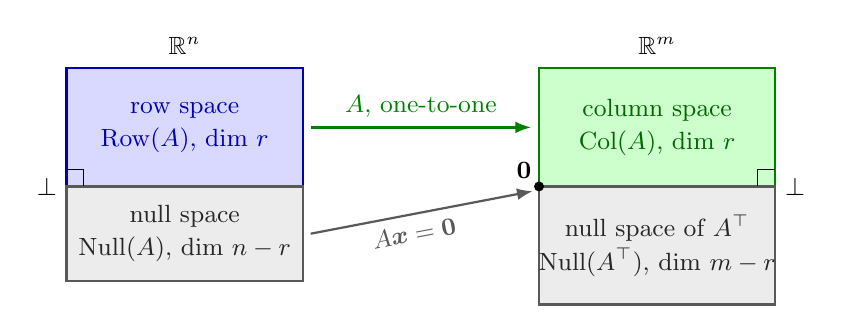
\begin{tikzpicture}[font=\small, >={Latex[length=2mm]}]
  % domain R^n
  \filldraw[blue!70!black, fill=blue!15, thick] (0,0) rectangle (3.0,1.5);
  \filldraw[gray!70!black, fill=gray!15, thick] (0,0) rectangle (3.0,-1.2);
  \node[blue!70!black, align=center] at (1.5,0.75) {row space\\[1pt] $\operatorname{Row}(A)$, dim $r$};
  \node[gray!30!black, align=center] at (1.5,-0.6) {null space\\[1pt] $\operatorname{Null}(A)$, dim $n-r$};
  \node[anchor=south] at (1.5,1.55) {$\mathbb{R}^n$};
  \draw[thin] (0.0,0.22) -- (0.22,0.22) -- (0.22,0);
  \node[anchor=east] at (0,0) {$\perp$};
  % codomain R^m
  \begin{scope}[xshift=6.0cm]
    \filldraw[green!50!black, fill=green!20, thick] (0,0) rectangle (3.0,1.5);
    \filldraw[gray!70!black, fill=gray!15, thick] (0,0) rectangle (3.0,-1.5);
    \node[green!40!black, align=center] at (1.5,0.75) {column space\\[1pt] $\operatorname{Col}(A)$, dim $r$};
    \node[gray!30!black, align=center] at (1.5,-0.75) {null space of $A^{\top}$\\[1pt] $\operatorname{Null}(A^{\top})$, dim $m-r$};
    \node[anchor=south] at (1.5,1.55) {$\mathbb{R}^m$};
    \draw[thin] (2.78,0) -- (2.78,0.22) -- (3.0,0.22);
    \node[anchor=west] at (3.0,0) {$\perp$};
    \fill (0,0) circle (1.8pt);
  \end{scope}
  % the map
  \draw[->, thick, green!50!black] (3.1,0.75) -- (5.9,0.75)
    node[midway, above] {$A$, one-to-one};
  \draw[->, thick, gray!70!black] (3.1,-0.6) -- (5.92,-0.06)
    node[pos=0.45, below, sloped] {$A\boldsymbol{x}=\boldsymbol{0}$};
  \node[anchor=south east, inner sep=2pt] at (5.98,0.02) {$\boldsymbol{0}$};
\end{tikzpicture}
\end{document}
